\vspace{-2mm}
\subsection{Relation Type Study}

 

\begin{figure}[t]
\centering
 
\includegraphics[width=5.5in]{submissions/Jing2024/figures/experiments/relation_analysis/legend.pdf}
\\\vspace{-6mm}
\subfloat[\textit{Averaged metrics} vs Head entity type]{
 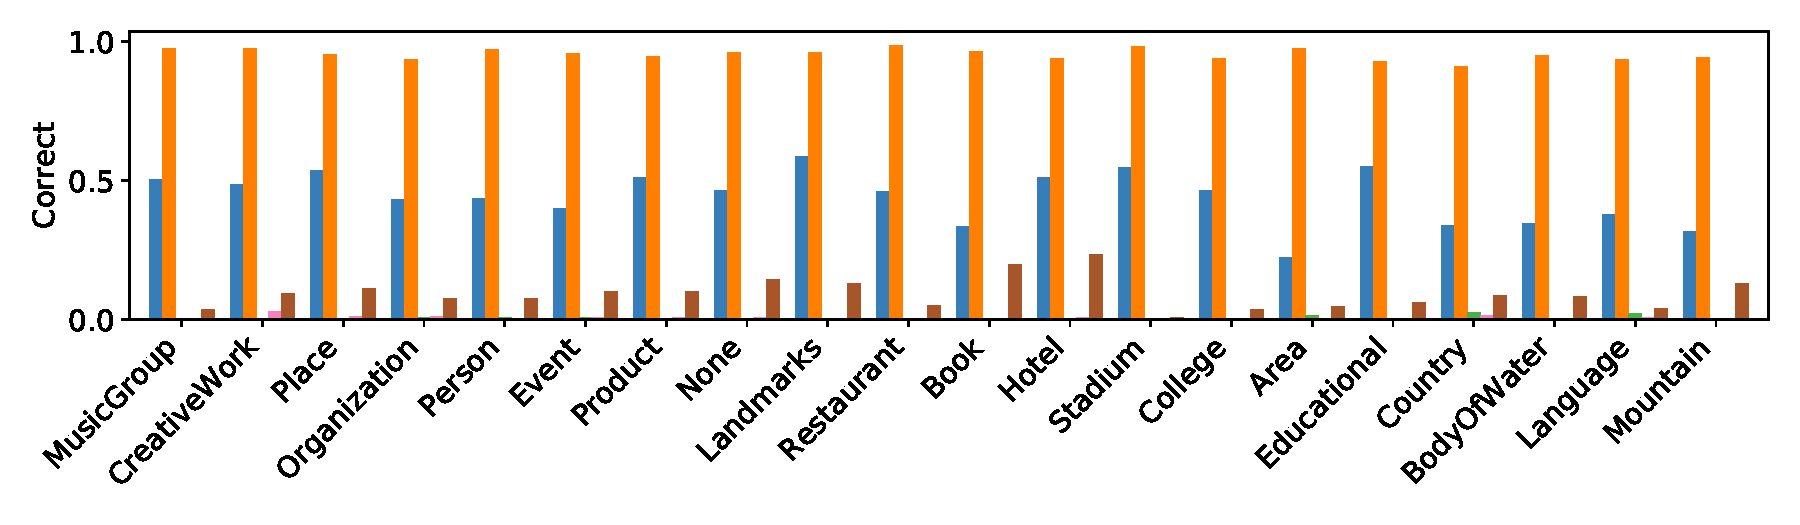
\includegraphics[width=5.5in]{submissions/Jing2024/figures/experiments/relation_analysis/correct_by_head_type.pdf}
 \label{fig:avg_by_head_type}
}\\
\vspace{-4mm}
\subfloat[\textit{Averaged metrics} vs Tail entity type]{
 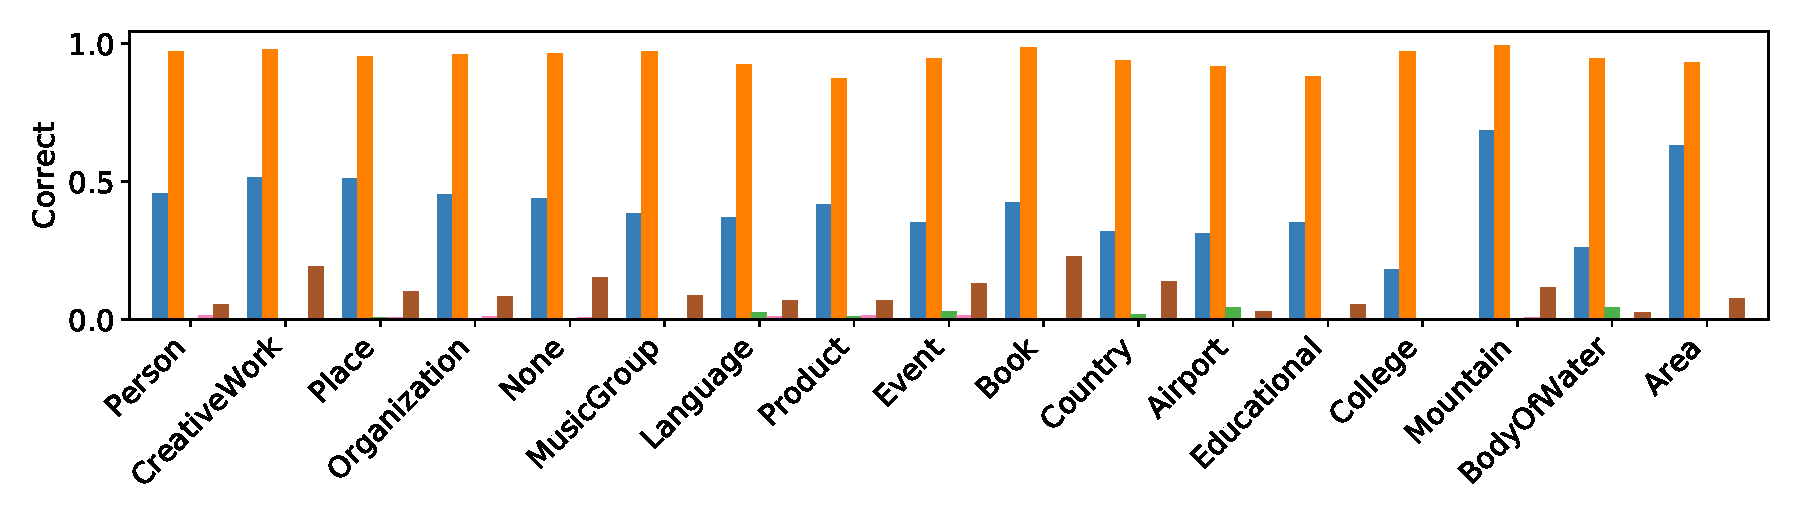
\includegraphics[width=5.5in]{submissions/Jing2024/figures/experiments/relation_analysis/correct_by_tail_type.pdf}
 \label{fig:avg_by_tail_type}
}
\vspace{-4mm}
\caption{The LLM's {\it averaged metrics} with respect to head entity types and tail entity types}
\vspace{-3mm}
\label{fig:avg_by_type}
\end{figure}


\label{exp:relation_type_study} 
There are more than 600 different relation types in the DBpedia knowledge graph, and each relation type has different characteristics. It is unclear if we directly compare the performance of the LLMs on different relation types.
Thus, to gain a better understanding of the LLM's performance, we first analyze the LLM's performance with respect to relation types. In DBpedia, most entities are associated with a \url{https://schema.org/} type. Thus, we can categorize the relations into different types by the triples they belong to. We denote a relation's head/tail entity type as the most frequent schema type of the head/tail entity of the triples associated with the relation.
 For example, the relation \texttt{birthPlace} is associated with triples like \texttt{(Barack Obama, birthPlace, Hawaii)}, and the head entity \texttt{Barack Obama} is associated with the schema type \texttt{Person}, and the tail entity \texttt{Hawaii} is associated with the schema type \texttt{Place}. Then, the relation's head entity type is \texttt{Person}, and tail entity type is \texttt{Place}.
 We then analyze the LLM's performance with respect to these relation types. We report the performance of the LLMs on different relation types, by taking the average of the 3 metrics, \textit{correctness}, \textit{truthfulness}, and \textit{informativeness}, for each relation type. We present the results in Figure~\ref{fig:avg_by_type}. Here, ``None'' refers to entities not linked to a schema type. We also present a detailed analysis of the LLM's performance with respect to head and tail entity types in Appendix~\ref{app:relation_type_study}.
We can observe variability in model performance across relation types, such as ``MusicGroup" and ``CreativeWork" achieving high scores while ``Area" and "Mountain" face lower performance, highlighting the diverse challenges in modeling different kinds of information. These performance differences suggest that the effectiveness of LLMs in handling structured knowledge heavily depends on the nature of the relations being modeled.
